%% TCC - Monografia
%% Ci\^{e}ncia da Computa\c{c}\~{a}o - LCMAT - CCT - UENF, 2018
%% 

\chapter{Arquitetura em camadas}\label{cap5}

\section{Criação do fluxo das arquiteturas}

Como todo projeto a ser desenvolvido, precisamos planejar e analisar todas as tecnologias, fluxos e informações sobre o que desejamos fazer. No desenvolvimento de software não é diferente, precisamos criar um fluxograma da arquitetura.

\subsubsection{Fluxograma da arquitetura em camadas}

Como já descrito no capítulo 2 sobre a arquitetura em camadas, onde serão usadas as camadas de \textbf{Presentation Layer} , \textbf{Business Layer}, \textbf{Service Layer}, \textbf{Persistence Layer} e \textbf{Database Layer}, teremos em nosso projeto essas mesmas partes da arquitetura, porém chamaremos aqui de Visualização, Controle, Serviço, Modelo e banco de dados. 

Descreveremos uma breve descrição do projeto que iremos desenvolver. O sistema será construído para uma Universidade, onde a quantidade de usuários é limitada a um nicho, pois para poder participar do sistema ela terá que seguir alguns requisitos como ter coeficiente de rendimento 7.0, então em uma Universidade com 6000 alunos e 1000 professores, podemos analisar que também é um sistema sazonal, onde terá uma carga um pouco maior em tempos de edital aberto, logo o pico de acesso será maior durante períodos específicos e nesse caso a arquitetura em camadas é ideal, não que para grandes acessos ela não seja uma boa escolha também, porém nesse caso em específico ela poderá ser mais fácil de se desenvolver, nesse caso também é interessante deixar claro que não será um sistema de código aberto, haja visto que o sistema é de propriedade da Universidade e coordenado pela Doutora Annabell. 

O projeto utilizará a linguagem de programação \textbf{Ruby} com o \textbf{framework Ruby on Rails}, e o banco de dados \textbf{PostgreSQL}, para armazenar nosso código, utilizaremos um repositório open source chamado Gitlab que nos ajudará a fazer um sistema automatizado com suporte a \textbf{continuous integration}, \textbf{continous deployment} e \textbf{continous delivery}. Utilizaremos o Heroku um famoso PaaS para não nos preocuparmos nesse momento com a infraestrutura.

\begin{figure}[htbp]
\hypertarget{arquitetura}{%
\caption{UML mostrando o fluxo da arquitetura baseada em camadas, pensando que é uma única base de código}
\begin{center}
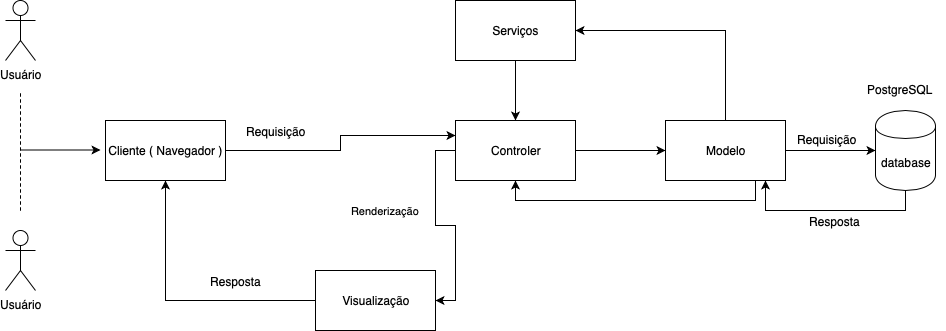
\includegraphics[width=15cm]{Monografia-FormatoLatex/Imagens/ArquiteturaEmCamadas.png}
\end{center}
}
\legend{Fonte: Criado pelo autor no site draw.io}
\label{fig:arquitetura-fluxograma}
\end{figure}

\subsection{Cliente ( Navegador )}

Toda interface que se pode visualizar os dados. Porém para a nossa aplicação utilizaremos os navegadores, mais especificamente o Chrome.

\subsection{Controller}

O controller é a parte da aplicação que intermediará o modelo e a visualização.

\subsection{Serviços}

A camada de serviço é um objeto simples Ruby que encapsula um conjunto de lógica de negócios, movida do controller ou até mesmo do modelo para ser ter configurações e regras mais focadas.

\subsection{Modelo}
A camada de modelo nos permite escrever todas as regras de negócio de uma aplicação. É também a camada que permite se comunicar com o banco de dados, executando assim os famosos CRUDs.

\subsection{Banco de dados}

A camada de modelo tem acesso ao banco de dados através da ORM. O ORM (Object Relational Mapper) é um mapeador relacional de objetos. Isso significa que você não precisa chamar manualmente o banco de dados, o ORM lida com isso para você.

\subsection{Visualização}

A camada de visualização é responsável por pegar as informações que o controller e representar essas informações. É importante informar que a camada de visualização pode representar os dados em diversos formatos, alguns: XML, CSV, JSON e HTML.

\section{Implementação da arquitetura em camadas}

Como a arquitetura em camadas tende a utilizar todas as partes do software em um único projeto, temos aqui nas pastas do Ruby on Rails pastas bem definidas para essas camadas. Caso queira ter acesso ao código fonte o mesmo está no link: https://gitlab.com/rdxinho/pibict é necessário a solicitação de acesso.


\subsection{Cliente ( Navegador )}

Como interface utilizaremos os navegadores para interagir com o sistema. O navegador faz uma requisição e recebe uma resposta e isso pode ficar mais claro utilizando o DevTools do Chrome. Na aba networking visualizamos diversas informações falaremos aqui algumas brevemente, pois não é o ponto focal do projeto. Nas figuras \ref{fig:devtools-waterfall} \ref{fig:devtools-ordem-de-arquivos} \ref{fig:devtools-status-barra}

\begin{figure}[htbp]
\hypertarget{arquitetura}{%
\caption{ Lista de todos os arquivos carregados para renderizar a página }
\begin{center}
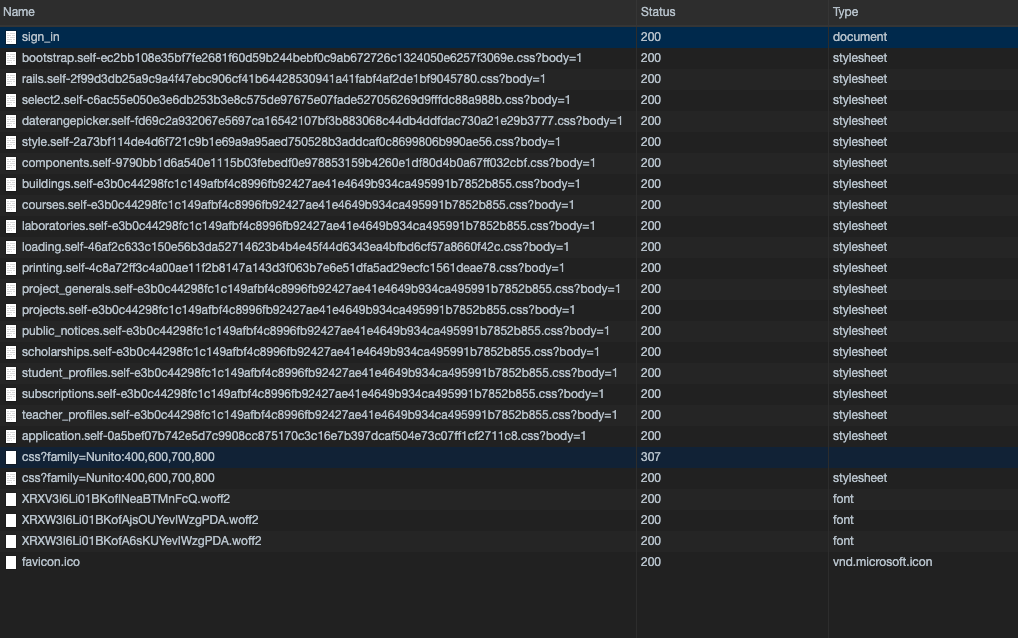
\includegraphics[width=15cm]{Monografia-FormatoLatex/Imagens/ordem-dos-arquivos-carregados.png}
\end{center}
}
\legend{Fonte: Criado pelo autor, uma imagem printada do navegador Chrome}
\label{fig:devtools-ordem-de-arquivos}
\end{figure}



\begin{figure}[htbp]
\hypertarget{arquitetura}{%
\caption{ Gráfico de carregamento dos arquivos }
\begin{center}
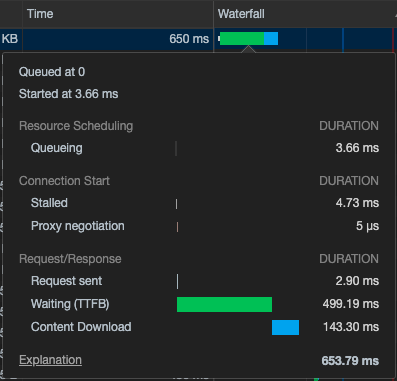
\includegraphics[width=15cm]{Monografia-FormatoLatex/Imagens/informacoes-do-waterfall.png}
\end{center}
}
\legend{Fonte: Criado pelo autor, uma imagem printada do navegador Chrome}
\label{fig:devtools-waterfall}
\end{figure}



\begin{figure}[htbp]
\hypertarget{arquitetura}{%
\caption{ Barra de status com algumas informações }
\begin{center}
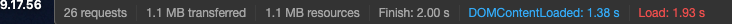
\includegraphics[width=15cm]{Monografia-FormatoLatex/Imagens/status-request-file-size.png}
\end{center}
}
\legend{Fonte: Criado pelo autor, uma imagem printada do navegador Chrome}
\label{fig:devtools-status-barra}
\end{figure}



\subsection{Controller}

O controller são responsáveis por orquestrar o modelo e a visualização. No framework Rails utilizamos uma pasta em \textbf{app/controllers} para adicionar todos os 'orquestradores' da nossa aplicação. É a responsável por receber um request e responder a um request.



\begin{figure}[htbp]
\hypertarget{arquitetura}{%
\caption{ Um código simples para ilustrar o código de um controller }
\begin{center}
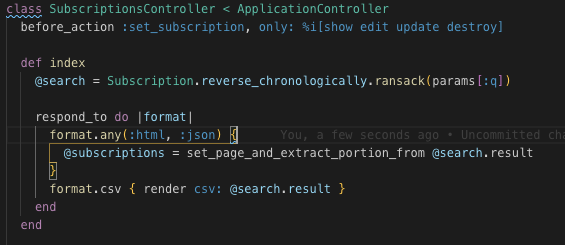
\includegraphics[width=15cm]{Monografia-FormatoLatex/Imagens/controller-camadas-exemplo.png}
\end{center}
}
\legend{Fonte: Criado pelo autor, uma imagem do código PIBICT}
\label{fig:controller-camadas}
\end{figure}


\subsection{Serviços}

Como a arquitetura baseada no modelo Model, View e Controller(MVC) enfrenta alguns problemas, adicionamos algumas camadas extras como por exemplo a camada de Serviços. Podemos criar diversos serviços com regras definidas baseada em uma determinada lógica de domínio. O controller tem uma responsabilidade muito bem definida, que é receber a requisição, verificar o que será feito, receber aquele dado e responder ao cliente. Quando ele (quem?) começa a ter lógica, já começamos a ver um espaço para a utilização de uma camada extra, que é a camada de serviço. Podemos verificar um código de serviço na figura \ref{fig:service-camadas}.


\begin{figure}[htbp]
\hypertarget{arquitetura}{%
\caption{ Um código simples para ilustrar o código de um serviço }
\begin{center}
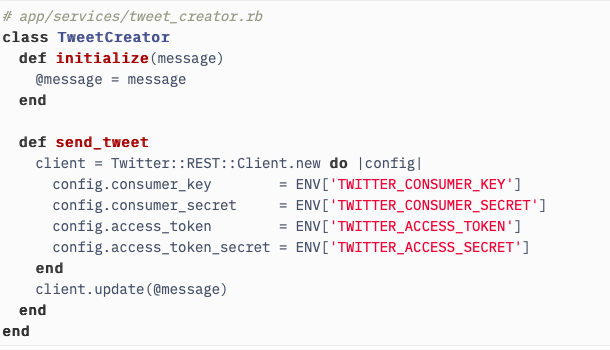
\includegraphics[width=15cm]{Monografia-FormatoLatex/Imagens/examplo-camada-service.png}
\end{center}
}
\legend{Fonte: Imagem retirada do link https://www.toptal.com/ruby-on-rails/rails-service-objects-tutorial }
\label{fig:service-camadas}
\end{figure}



\subsection{Modelo}
O Ruby on Rails também nos dá uma estrutura de pasta pronta para receber os modelos. Essa estrutura fica em \textbf{app/models}.

\begin{figure}[htbp]
\hypertarget{arquitetura}{%
\caption{ Um código simples para ilustrar o código do modelo }
\begin{center}
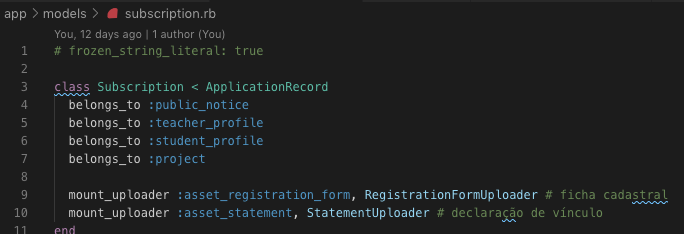
\includegraphics[width=15cm]{Monografia-FormatoLatex/Imagens/exemplo-model.png}
\end{center}
}
\legend{Fonte: Imagem retirada do link https://www.toptal.com/ruby-on-rails/rails-service-objects-tutorial }
\label{fig:service-model}
\end{figure}


\subsection{Banco de dados}

O projeto utilizará o banco de dados PostgreSQL.

\subsection{Visualização}

Os dados serão representados utilizando o HTML, CSS e Javascript. O Ruby on Rails nos dá também o ERB para dinamicamente podermos fazer essas junção dos dados retornados pelo controller.